\title{Computer Logic and Digital Circuit Design: Midterm 1}
\author{Dr. Jordan Hanson - Whittier College Dept. of Physics and Astronomy}
\date{\today}
\documentclass[10pt]{article}
\usepackage[a4paper, total={18cm, 27cm}]{geometry}
\usepackage{outlines}
\usepackage{graphicx}
\begin{document}
\maketitle

\section{Chapter 1 - Introductory Concepts}
\begin{figure}[ht]
\centering
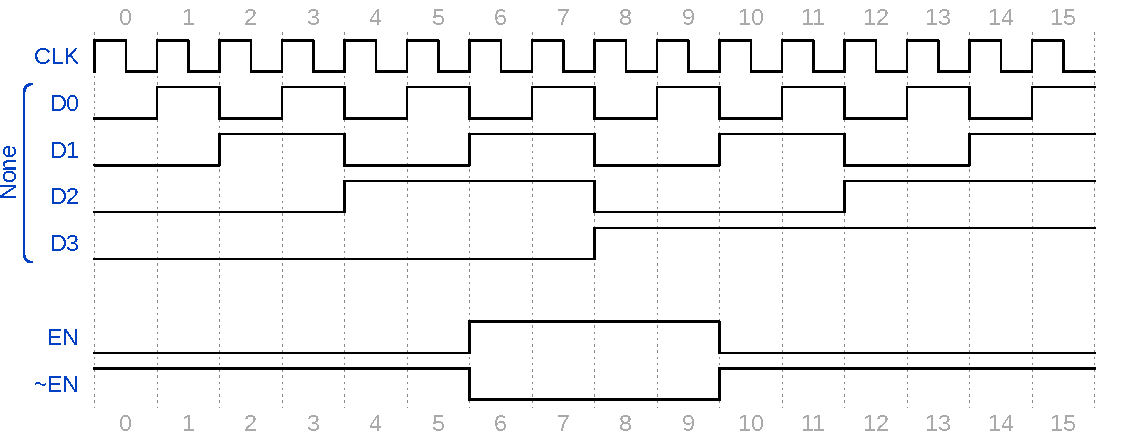
\includegraphics[width=0.6\textwidth]{timingExample6.pdf}
\caption{\label{fig:timing1} A timing diagram including a clock signal (CLK), a 4-bit parallel data stream (D0-D3), and enable/disable signals (EN/$\sim$EN).}
\end{figure}
\begin{enumerate}
\item Consider Fig. \ref{fig:timing1}. (a) What is the duty cycle of each $D_{\rm i}$ signal? (b) Consider the bitstreams of $D_{\rm i}$.  What does the sequence of numbers represent? \\ \vspace{1.0cm}
\item (a) Create the timing diagram representing the output of an XOR gate with $D_0$ and $D_1$ as inputs. (b) Do the same for $D_2$ and $D_3$.  (c) Finally, create the timing diagram representing the output of a 3-input AND gate with the XOR gates from parts (a) and (b), and the EN signal as inputs. \\ \vspace{2.0cm}
\item Suppose $D_i$ represents parallel data with a clock frequency of 4 MHz.  (a) What is the total bitrate (bits per second)?  (b) What would be the bit rate if the system was serial instead of parallel? \\ \vspace{0.5cm}
\end{enumerate}

\section{Chapter 2 - Number Systems, Operations, and Codes}

\begin{enumerate}
\item Convert to binary: (a) 1024 (b) 0xBBBB (c) -2048 \\ \vspace{1cm}
\item Convert to hex: (a) 65535 (b) 1000100010001000 \\ \vspace{1cm}
\item \textbf{Design problem.}  Consider the angular shaft encoder in Fig. \ref{fig:grayCode}.  The IR emitter/detector detects IR light reflected from white sectors, while the dark sectors absorb the light.  The sectors are encoded in binary.  For example, starting from inner sectors and reading outward, dark-dark-light is translated to state 001 by the detector.  If the shaft rotates 45 degrees, the detector records a state change.  (a) If the initial state is 000 and the shaft rotates 360 degrees, how many bit changes occur?  (b) How many bit changes would occur if the shaft position was encoded in gray code?  (c) Draw the correct face of the shaft encoder, encoded in 3-bit gray code instead of binary\footnote{Caution: I believe the figure in the textbook contains errors.} (c) If 45 degrees is the angular precision with 3-bit gray code, what is the angular precision with 8 bit gray code? \\ \vspace{2cm}
\end{enumerate}
\begin{figure}[hb]
\centering
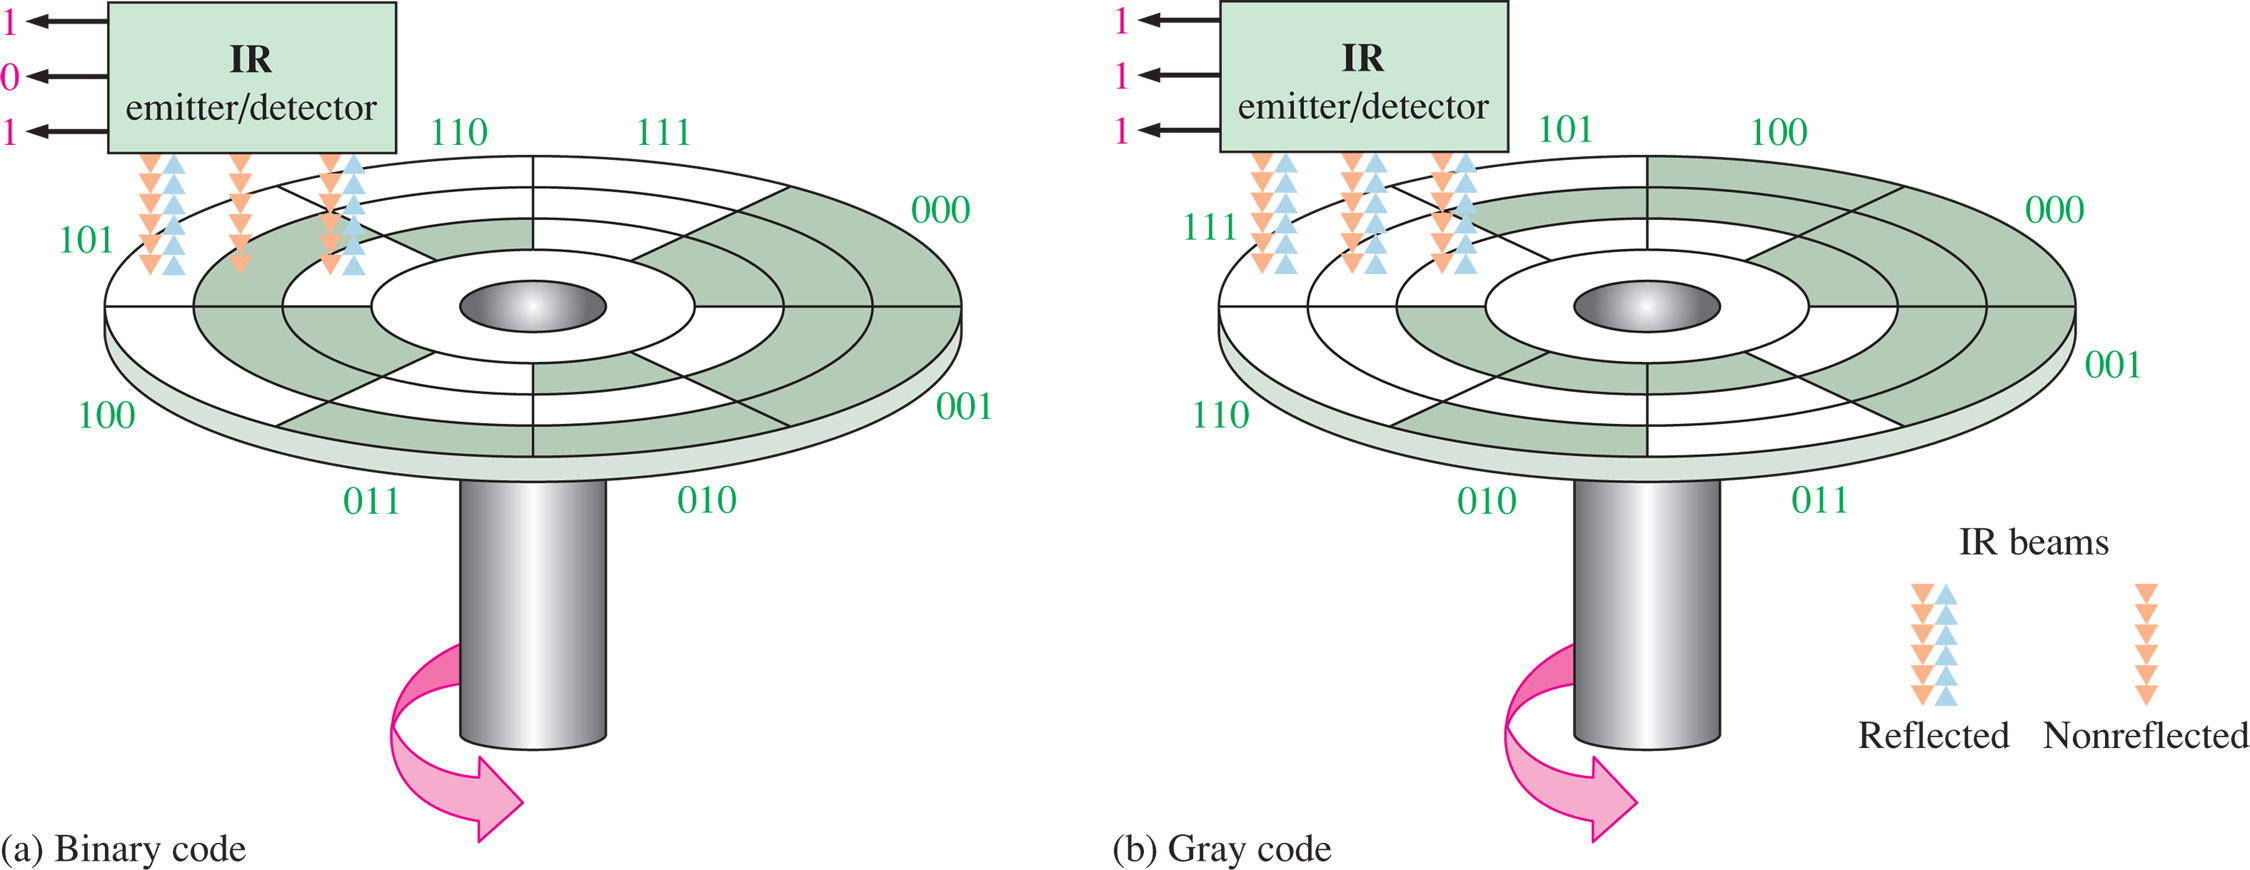
\includegraphics[width=0.33\textwidth,trim=0cm 0cm 12cm 0cm,clip=true]{gray_code_shaft.jpg}
\caption{\label{fig:grayCode} A gray code shaft encoder, or angular encoder, reports the angular position of an object digitally, using the gray code.}
\end{figure}

\section{Chapter 3 - Logic Gates}
\begin{figure}[ht]
\centering
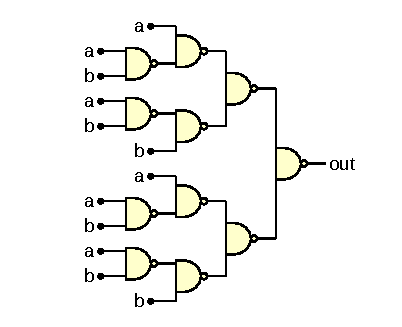
\includegraphics[width=0.25\textwidth]{gateExample5.pdf}
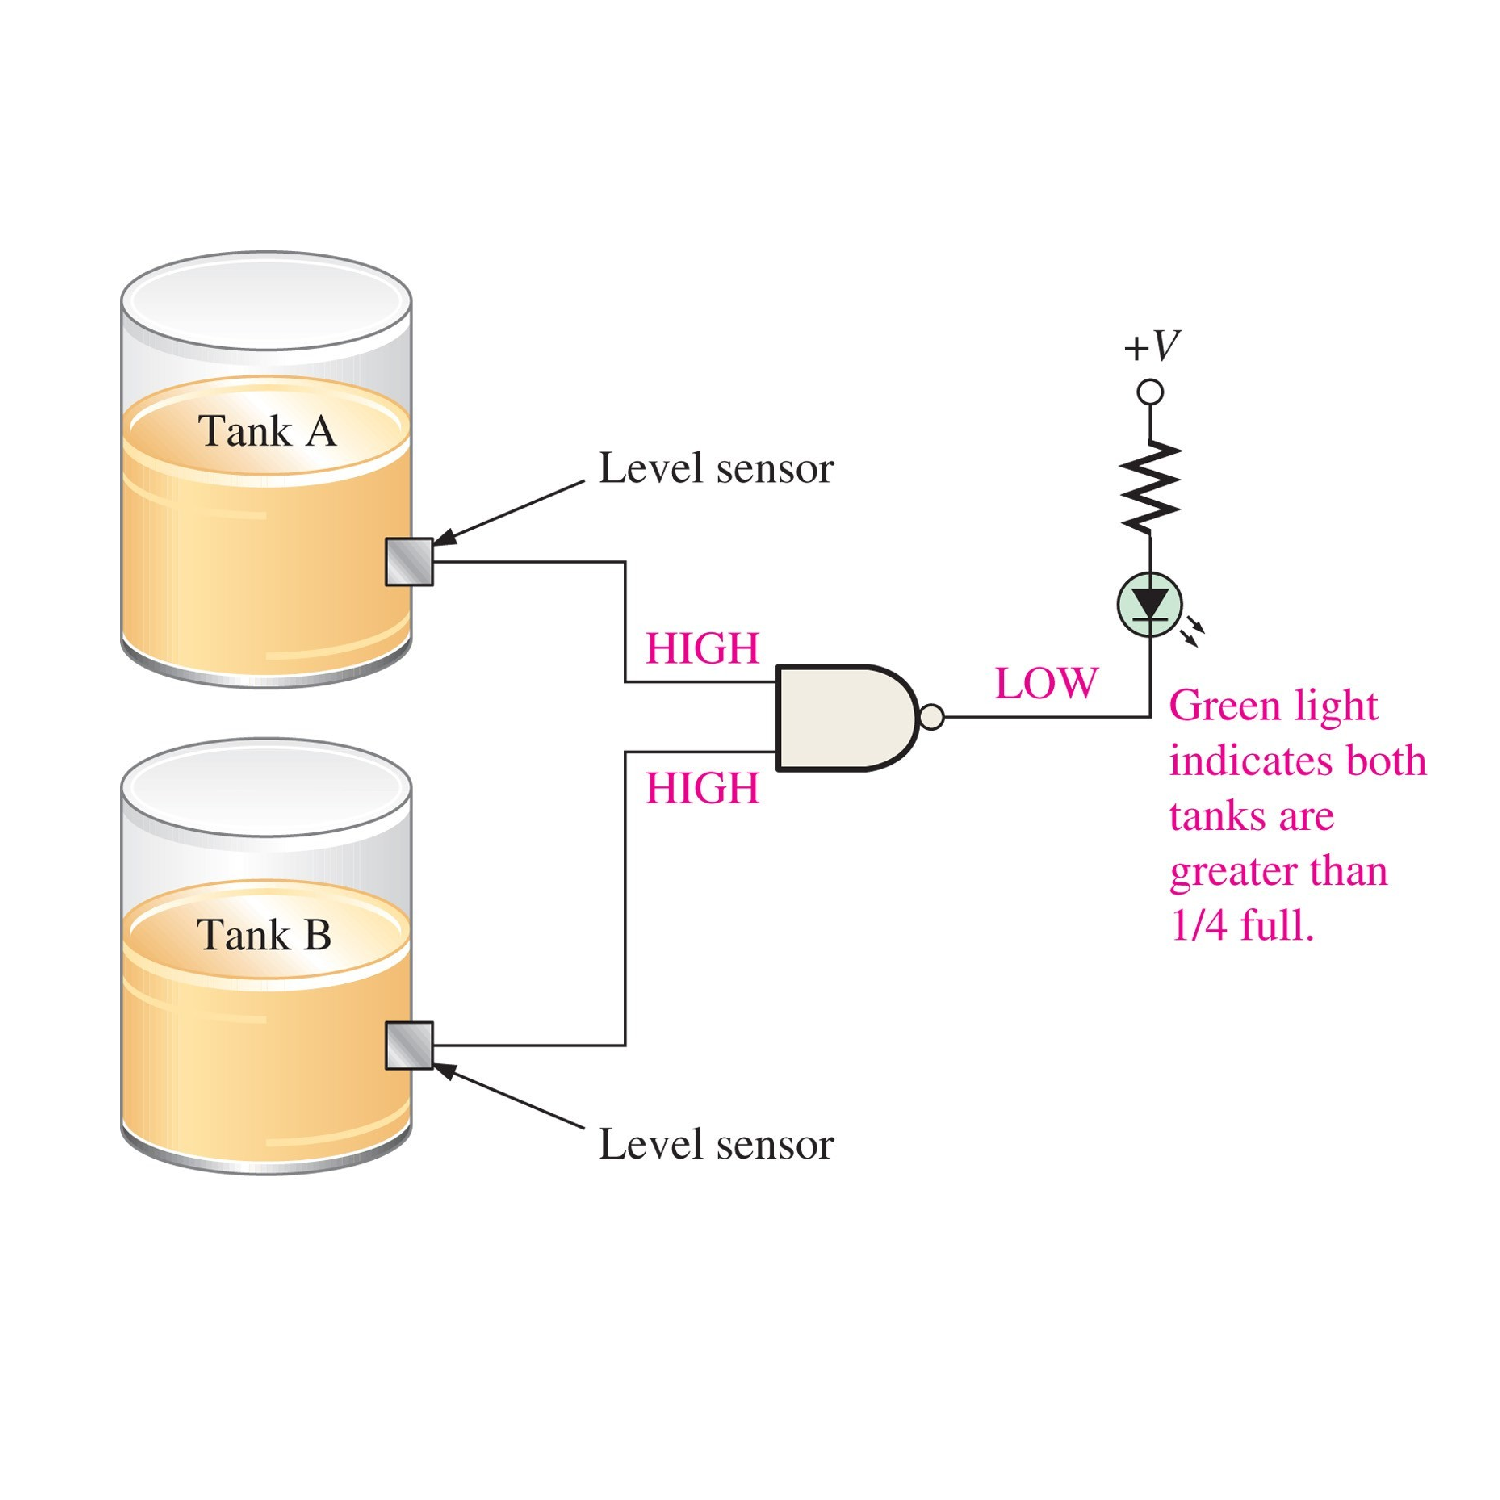
\includegraphics[width=0.25\textwidth]{gateExample6.pdf}
\caption{\label{fig:gates1} (Left) A logic gate combination.  (Right) A liquid tank-level system built from a NAND gate.}
\end{figure}
\begin{enumerate}
\item Generate the simplified logic expression and truth table for Fig. \ref{fig:gates1}, left.  What do you call this type of gate? \\ \vspace{1.5cm}
\item Suppose signals $D_{\rm 0}$ and $D_{\rm 1}$ in Fig. \ref{fig:timing1} are connected to $a$ and $b$ in Fig. \ref{fig:gates1}, left.  Generate the timing diagram. \\ \vspace{1cm}
\item \textbf{Design problem.}  A liquid tank system is depicted in Fig. \ref{fig:gates1} (right).  The sensors are HIGH when the liquid is above the level.  (a) Create and display a red LED system that activates when both tanks are \textit{below} the level.  (b) Create and display a yellow LED system that activates when one tank is below and one tank is above the level.  (c) Add a third tank with two pipes guiding liquid to tanks A and B.  Each pipe should have a valve.  Add logic that opens the correct valve so as to fill only the low tank until it is no longer below the level.  \\ \vspace{5cm}
\end{enumerate}

\section{Chapter 4 - Boolean Algebra and Logic Simplification}

\begin{enumerate}
\item Suppose an investment firm manages a portfolio with shares in four stocks, labled A through D.  The companies corresponding to stocks A through D are labeled \textit{inactive} or \textit{active} by the firm, based on productivity information.  The firm notices that returns (profits) for the portfolio increase under the following conditions:
\begin{itemize}
\item All four companies are active, or ...
\item Companies A and B are inactive, while companies C and D are active, or ...
\item Company A is inactive, while companies B, C, and D are active, or ...
\item Company B is inactive, while companies A, C, and D are active.
\end{itemize}
(a) Develop a S-SOP expression for $X$, the portfolio's state.  If profit is increasing, label the output ON, and label it OFF if profit is decreasing. (b) Use a domain-4 Karnaugh map to simplify the S-SOP expression. (c) Based on your analysis, which stock or stocks should be eliminated from the portfolio?  \\ \vspace{2.5cm}
\item A circuit contains three main branches leading to one output.  The output is observed to \textbf{fail} under the following conditions below.  (a) Use the domain-3 Karnaugh map to determine the conditions under which it does succeed, and write an S-SOP expression for the circuit. (b) Draw the circuit using gates.
\begin{itemize}
\item A: false, B: false, C: false
\item A: false, B: true, C: false
\item A: true, B: true, C: false
\item A: true, B: false, C: false
\item A: false, B: true, C: true
\item A: true, B: true, C: true
\end{itemize}
\end{enumerate}

\clearpage

\section{Chapter 5 - Combinatorial Logic Analysis}
\label{sec:comb}
\begin{figure}[ht]
\centering
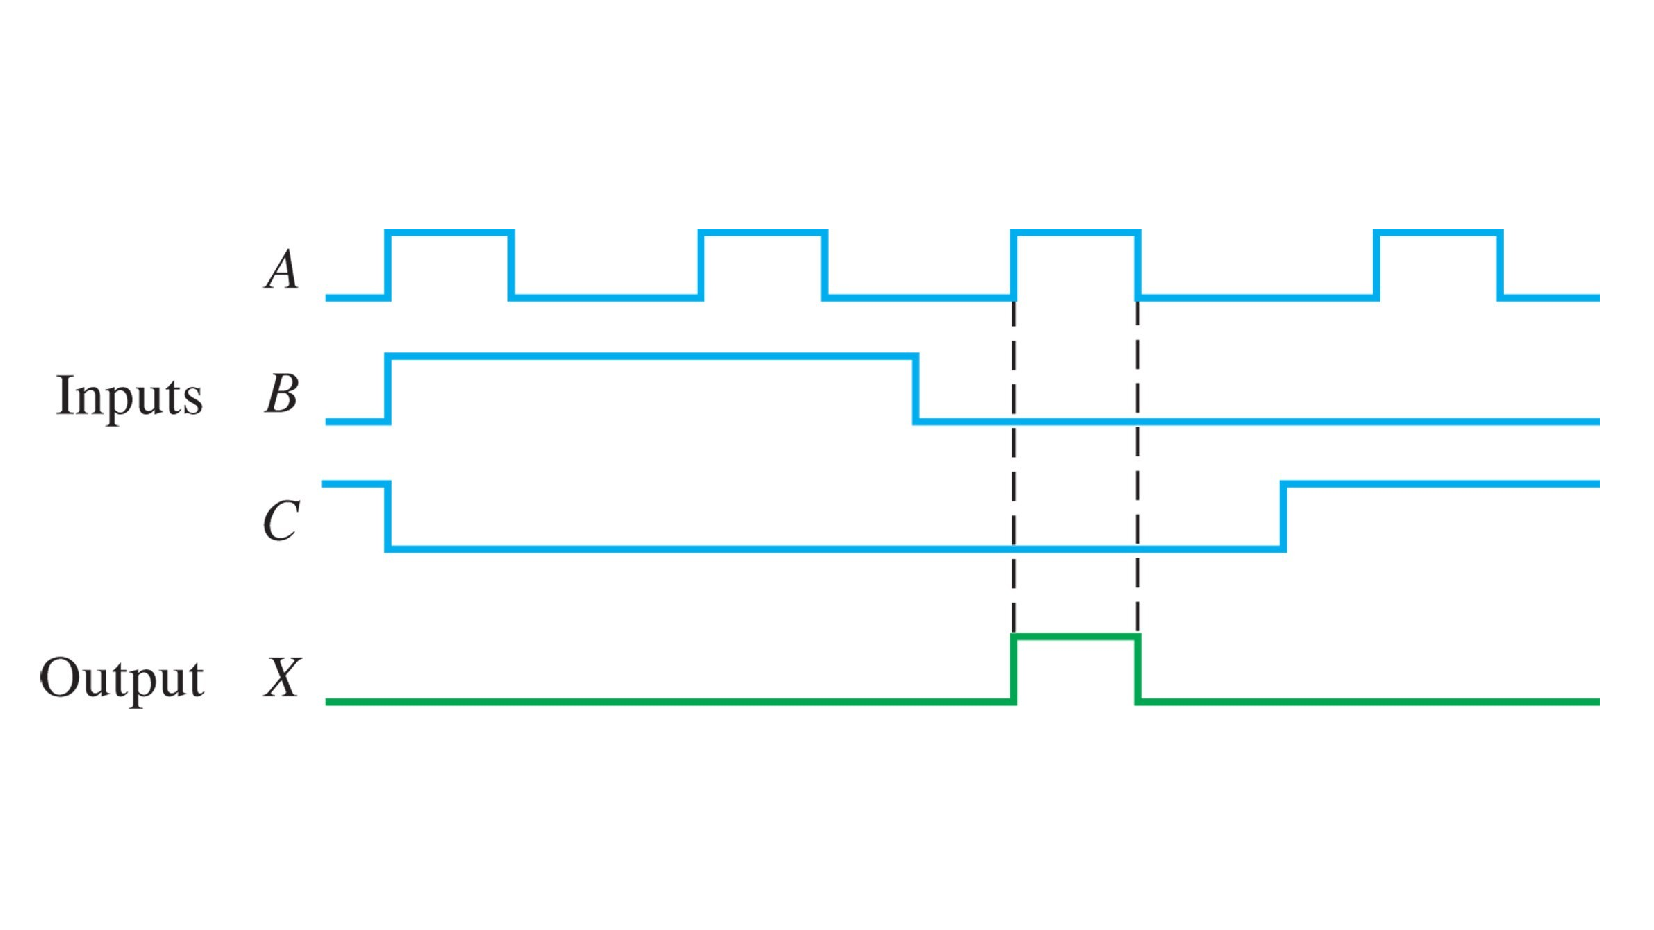
\includegraphics[width=0.4\textwidth,trim=0cm 3cm 0cm 2cm,clip=true]{timingExample7.pdf} \hspace{1cm}
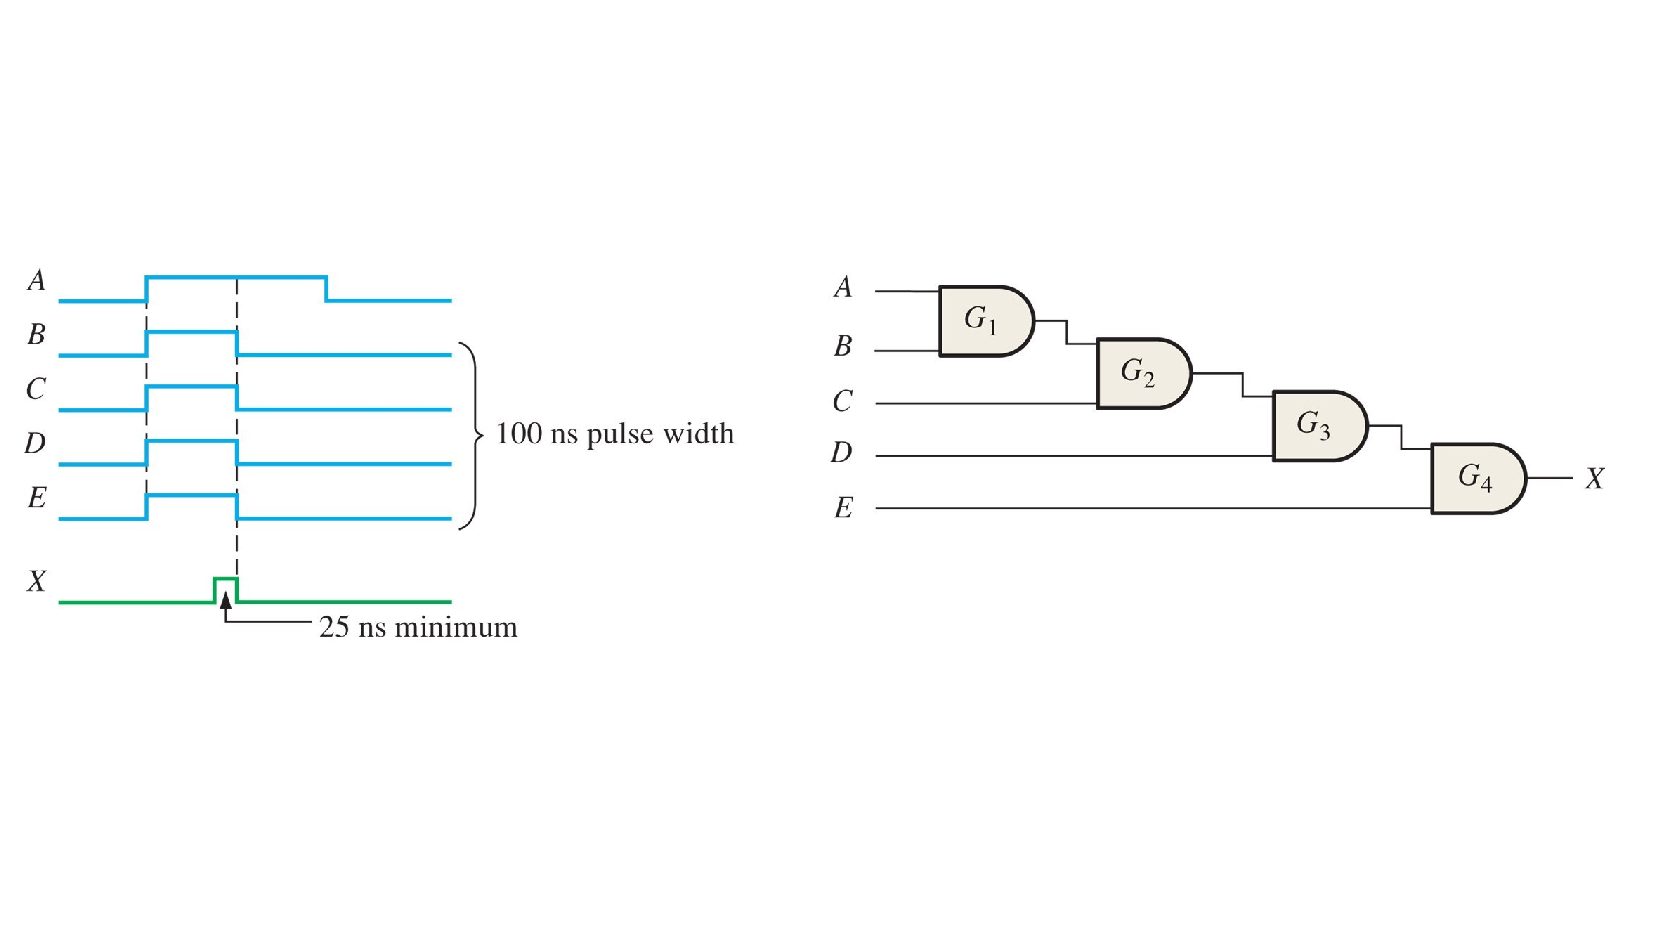
\includegraphics[width=0.5\textwidth,trim=0cm 4cm 0cm 2cm,clip=true]{bonus.pdf}
\caption{\label{fig:timing3} Diagrams for Sec. \ref{sec:comb}. (Left) Inputs are ABC, and the output is X. (Right) The inputs are ABCDE, and the output is X.}
\end{figure}
\begin{enumerate}
\item For the input waveforms shown in Fig. \ref{fig:timing3} (left), what logic circuit will generate the output waveform? \\ \vspace{2cm}
\item \textbf{Bonus}: Assumming a propagation delay of 10 ns through each gate in Fig. \ref{fig:timing3}, determine if the \textit{desired} output waveform X will be generated.  The desired output is a pulse with a minimum width of 25 ns.
\end{enumerate}

\end{document}